\documentclass[fancyhdr, oneside, UTF8, openany]{ctexbook}

\usepackage[a4paper, left=2.1cm, right=2.1cm, top=2.1cm, bottom=2.1cm]{geometry}
\usepackage{graphicx}
\usepackage{comment}
\usepackage{fancyvrb}
\usepackage{amsmath}
\usepackage{amssymb}
\usepackage{tabularx}
\usepackage{fancyhdr}
\usepackage{pdfpages}
\usepackage{xurl}

\renewcommand\CJKecglue{}

\ctexset{
  today=old,
  chapter={
    name={第,章},
    format+=\LARGE,
    number=\arabic{chapter}}}

\def\header{九章论文}

\newcommand\printabstract{
    \addcontentsline{toc}{chapter}{摘要}
    \begin{center}
    \LARGE\heiti{}摘要
    \end{center}}

\newcommand\printenglishabstract{
    \addcontentsline{toc}{chapter}{ABSTRACT}
    \begin{center}
    \LARGE\textbf{ABSTRACT}
    \end{center}}


\begin{document}

% 封面导入, 可使用其他排版软件生成的PDF(可包含多页).
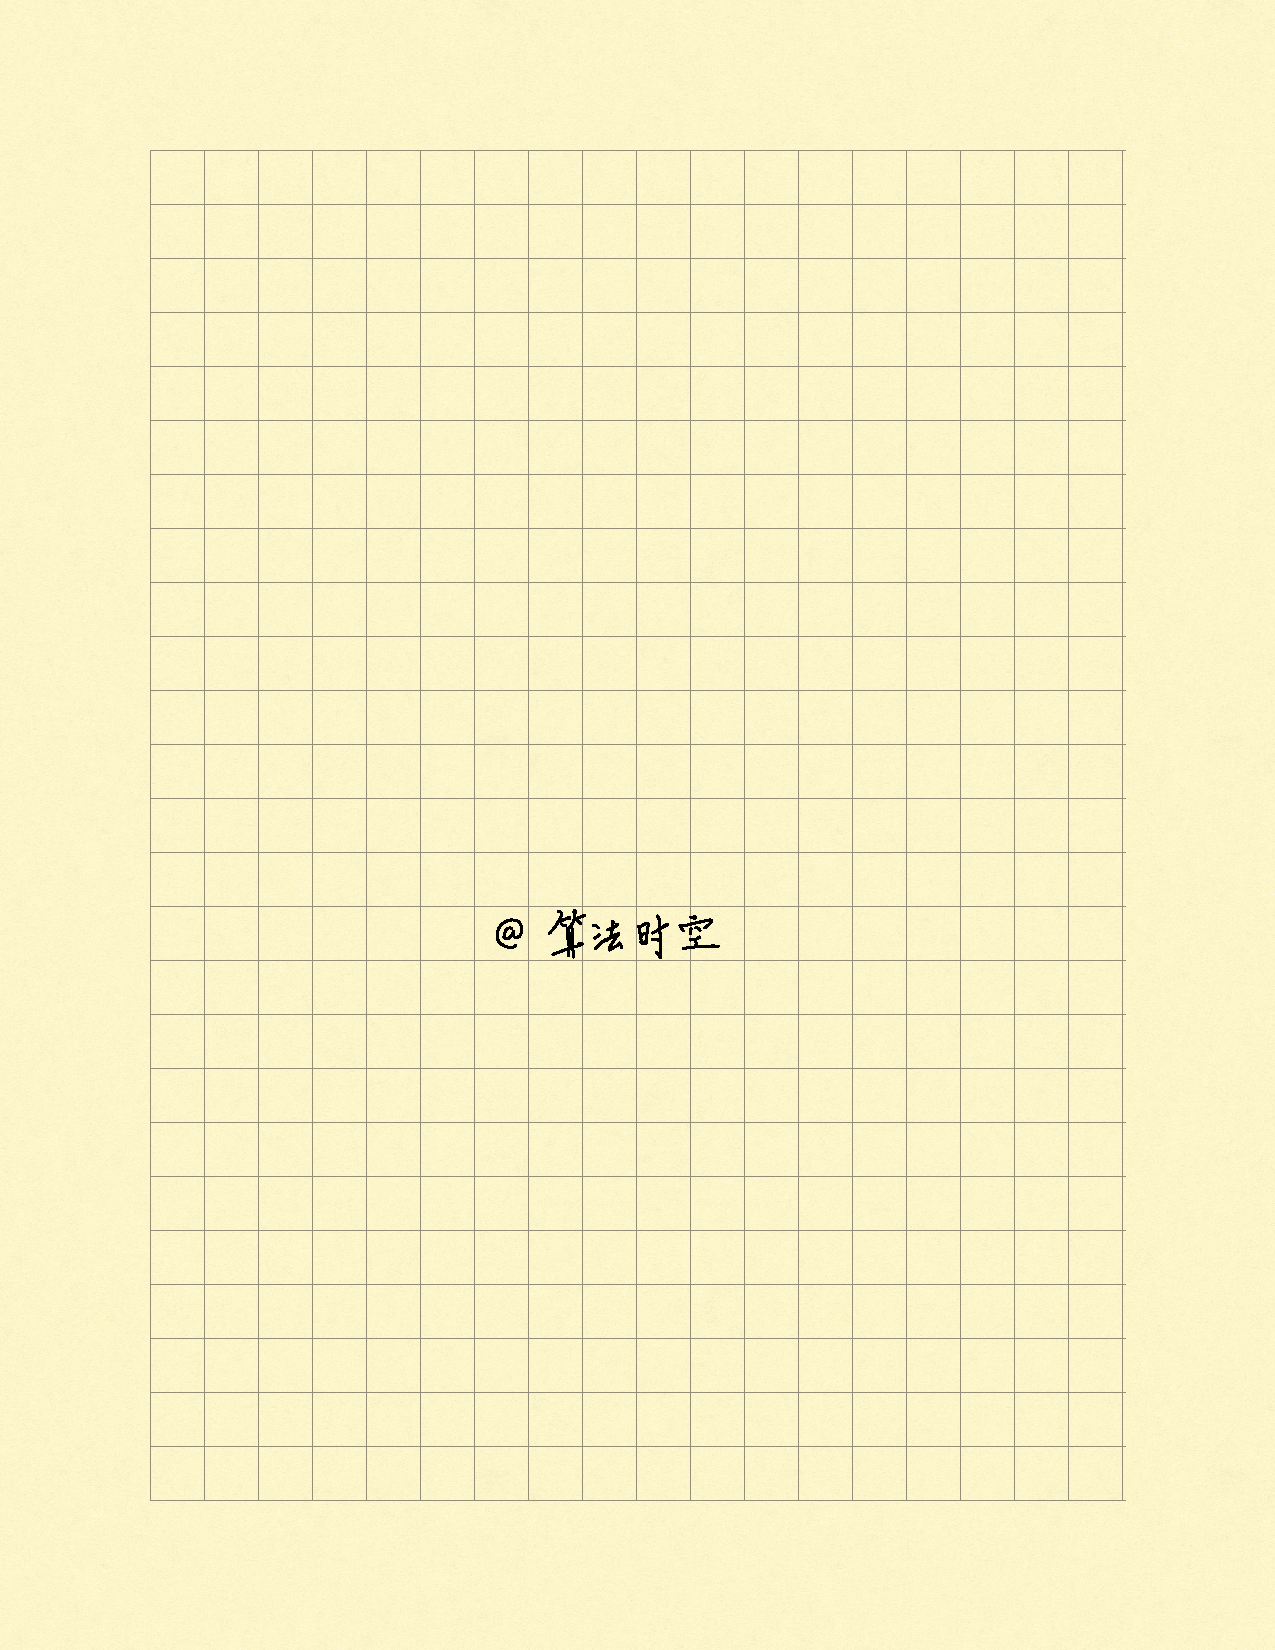
\includepdf[pages=-]{cover.pdf}

% 目录
\pagestyle{empty}
\tableofcontents
\thispagestyle{empty}
\newpage

% 摘要
% 中文摘要设定
\newpage
\pagestyle{empty}
\pagenumbering{Roman}
\setcounter{page}{1}

\printabstract

% 中文摘要

简单明了.

\noindent{\heiti{}关键词}\textbf{:~}X; Y; Z

% 英文摘要设定
\newpage

\printenglishabstract

% 英文摘要

Clear \& Simple.

\noindent\textbf{Keywords:~}X; Y; Z

% 正文部分设定
\newpage
\pagestyle{fancy}
\fancyhead[L,R]{}
\fancyhead[C]{\header}
\fancyfoot[C]{\thepage}
\pagenumbering{arabic}
\setcounter{page}{1}

% 九章
\chapter{结构}

\section{节}

\subsection{小节}
\chapter{文字}

书写

\newpage

用心

\chapter{公式}

\begin{equation}
\log(n!) = \Theta(n\log{n})
\end{equation}
\chapter{图片}

\begin{figure}[!hbtp]
    \centering
    
\includegraphics[width=.8\textwidth]{books.jpg}
    \caption{算法三部曲.}
    \label{fig:books}
\end{figure}
\chapter{表格}

\begin{table}[!hbtp]
\centering
\begin{tabular}{|c|l|r|}
\hline
    & Books                         &     \\ \hline
1   & Introduction to Algorithms    & 3 \\
2   & The Algorithm Design Manual   & 2 \\
3   & Algorithms                    & 4 \\
\hline
\end{tabular}
\caption{算法三部曲}
\label{tab:trilogy}
\end{table}
\chapter{引用}
\chapter{版式}
\chapter{辅助}
\chapter{进阶}

\chapter*{致谢}
\addcontentsline{toc}{chapter}{致谢}

感谢Donald E. Knuth和Leslie Lamport, 感谢\TeX{}和\LaTeX{}.
% 为了简单起见, 我们不使用BibTeX.

\begin{thebibliography}{0}
\addcontentsline{toc}{chapter}{参考文献}

% 每条参考文献的名字就是作者名字或者多人全部字母的缩写, 若重复用年份区别.

\bibitem{SX}
Steven S. Skiena [著], 谢勰 [译]. 算法设计指南 (第2版) [M]. 北京: 清华大学出版社, 2017.

\end{thebibliography}


\end{document}